%-----------------------------------------------------------------------------%
% Document class
%-----------------------------------------------------------------------------%
\documentclass[a4paper,12pt,onecolumn,final]{article}
%-----------------------------------------------------------------------------%
% Geometry package for setting page margins
%-----------------------------------------------------------------------------%
\usepackage[paper=a4paper,vscale=0.8,hscale=0.85,centering]{geometry}
%-----------------------------------------------------------------------------%
% Helvet package for font
%-----------------------------------------------------------------------------%
\usepackage[scaled=0.92]{helvet}
\renewcommand{\familydefault}{\sfdefault}
%-----------------------------------------------------------------------------%
% Include special packages here
%-----------------------------------------------------------------------------%
\usepackage{amsmath,amsfonts,amssymb}
\usepackage{xcolor}
\usepackage{graphicx}
\usepackage{hyperref}
\usepackage{listings}
\lstset {backgroundcolor=\color{black!5}, basicstyle=\footnotesize, stringstyle=\color{red}, commentstyle=\color{green!50!black}, basicstyle=\footnotesize\ttfamily, keywordstyle=\color{blue}, 
}
%-----------------------------------------------------------------------------%


%-----------------------------------------------------------------------------%
\begin{document}
%-----------------------------------------------------------------------------%


%-----------------------------------------------------------------------------%
\noindent
\begin{tabular}{|p{0.2\textwidth}|p{0.75\textwidth}|}
\hline
\textbf{G14CAM} & \textbf{Computational Applied Mathematics}
\\
2017--2018 & \textcolor{red}{Coursework 1 Part C}
\\
\hline
\textbf{Name} & \textcolor{red}{Ella Taylor}
\\ 
\textbf{Student ID} & \textcolor{red}{429052}
\\ 
\textbf{Date} & \today
\\
\hline
\textbf{Existing codes} & \textcolor{red}{Names of approved existing codes that you used}
\\
\hline
\end{tabular}
%-----------------------------------------------------------------------------%
% \textcolor{red}{LaTeX instruction: This TeX-file template can be compiled using PDFLaTeX.}
%-----------------------------------------------------------------------------%
\section*{Problem 1}
\subsection*{Problem 1.a}
Type your solution here, or upload hand written material
% \includegraphics[width=0.5\textwidth]{HandWrittenProblem1.pdf}

\subsection*{Problem 1.b}
\begin{lstlisting}[language=C++]
#include <iostream>
#include <cmath>
#include <cassert>

double f1(double x)
{
const double pi = 3.14159265358979323846;
return (1.0/18.0)*pow(x,4) - sin(pi*x/6.0);
}

double GQ1(double a, double b)
{
assert(a < b);
//Mapping Xi on to x using x = (b-a)/2 * Xi + (a+b)/2
//Integral approx equal to 2*f(0) for integrating between -1,1.
// Xi = 0 the x = (a+b)/2
//GQ1 = 2(b-a)/2 *f((a+b)/2)= (b-a)*f((a+b)/2)

return (b-a)*f1((a+b)/2);
}

int main()
{
const double a = 0.0;
const double b = 3.0;

double GQ_1;

GQ_1 = GQ1(a,b);

std::cout<<"GQ1 = "<<GQ_1<<"\n";

return 0;
}

\end{lstlisting}%

\subsection*{Problem 1.c}
\begin{lstlisting}[language=C++]

#include <cmath>
#include <cassert>
#include <iostream>

double f1(double x)
{
const double pi = 3.14159265358979323846;
return (1.0/18.0)*pow(x,4) - sin(pi*x/6.0);
}

double GQ3(double a, double b)
{
assert(a < b);
//Mapping Xi on to x using x = (b-a)/2 * Xi + (a+b)/2
//GQ3 = 5/9 * f(-sqrt(3/5)) + 8/9 * f(0) + 5/9  * f(sqrt(3/5))
//f(x) = 1/18 * pow(x,4) - sin(pi x /6)
//sin functions cancel as odd
double x[3];
x[0] = -sqrt(3.0/5.0);
x[1] = 0;
x[2] = sqrt(3.0/5.0);

double Xi[3];
for (int i=0; i<3; i++)
    {
    Xi[i] = x[i]*(b-a)/2.0 + (a+b)/2.0;
    }

return ((b-a)/2.0) * ( (5.0/9.0) * f1(Xi[0]) +(8.0/9.0) * f1(Xi[1]) + 
(5.0/9.0) * f1(Xi[2]) );
}

int main()
{
const double a = 0.0;
const double b = 3.0;

double GQ_3;

GQ_3 = GQ3(a,b);

std::cout<<"GQ3 = "<<GQ_3<<"\n";

return 0;
}

\end{lstlisting}%

%-----------------------------------------------------------------------------%
\section*{Problem 2}
\subsection*{Problem 2.a}
\begin{lstlisting}[language=C++]
#include <cmath>
#include <iostream>
#include <iomanip>

double f2(double x)
{
return tanh(100.0*(x-2.0)) * ((3.0-x)/10.0) * pow(pow(x,2)-x*pow(2,0.5)+
0.5005,0.5);
}


double CGQ1(int n, double a, double b)
{
double h = (b-a)/(double)(n);
double sum = 0;
double Xi;

//f = (tanh(100(x-2)))((3-x)/10)sqrt(x^2 - x sqrt(2)+ 0.5005)

for(double i = a; i<b; i = i+h)
    {
    Xi = (2.0 * i + h)/2.0;
    sum = sum + h * f2(Xi);
    }

return sum;
}

double CGQ3(int n, double a, double b)
{
double sum = 0.0;
double h = (b-a)/((double)(n));

double x[3];
x[0] = -sqrt(3.0/5.0);
x[1] = 0;
x[2] = sqrt(3.0/5.0);

double Xi[3];

//f = (tanh(100(x-2)))((3-x)/10)sqrt(x^2 - x sqrt(2)+ 0.5005)

for (double i = a; i<b; i = i+h)
    {

    for (int j=0; j<3; j++)
    {
    //mapping points on to interval [-1,1]
    Xi[j] = x[j]*h/2.0 + (2.0*i+h)/2.0;
    }

    sum = sum + (h/2.0)*( (5.0/9.0)*f2(Xi[0]) + (8.0/9.0)*f2(Xi[1]) + 
    (5.0/9.0)*f2(Xi[2]));
    }

return sum;
}

int main()
{
int n; //n is number of intervals
double h;
const double a = 0;
const double b = 3;

std::cout<< "N"<<std::setw(20)<<"h"<<std::setw(30)<<"CGQ1"<<
std::setw(35)<<"CGQ3"<<std::endl;
std::cout<<"--------------------------------------------
----------------------------------------------"<<std::endl;

for (int i=0; i<=7; i++)
{
n = pow(2,i);
h = (b-a)/n;
std::cout<<n<<std::setw(20)<<h<<std::setw(30)<<
CGQ1(n,a,b)<<std::setw(35)<<CGQ3(n,a,b)<<std::endl;
}

return 0;
}

\end{lstlisting}%
%
\begin{tabular}{cc|cc}
 $N$ & $h$ & $\mathrm{CGQ}_1$ & $\mathrm{CGQ}_3$
\\
\hline
 $1$ & $3$ & -0.356944 & -0.185565
\\
 $2$ & $\tfrac{3}{2}$ & 0.157268 & -0.0754361
\\
 $4$ & $\tfrac{3}{4}$ & -0.168996 & -0.11855
\\
 $8$ & $\tfrac{3}{8}$ & -0.0737691 & -0.102471
\\
 $16$ & $\tfrac{3}{16}$ & -0.123251 & -0.110649
\\
 $32$ & $\tfrac{3}{32}$ & -0.100556 & -0.106934
\\
 $64$ & $\tfrac{3}{64}$ & -0.109829 & -0.108087
\\
 $128$ & $\tfrac{3}{128}$ & -0.107711 & -0.10793
\\

\end{tabular}

\subsection*{Problem 2.b}
\begin{lstlisting}[language=C++]
#include <iostream>
#include <cmath>
#include <iomanip>

double CGQ1(int n, double a, double b);
double CGQ3(int n, double a, double b);

double adapt_int(double a, double b, double tau)
{
int n = 1; //number of  intervals
int n_new;
int N = 1000; //max number of mesh points
int counter = 0;
double Est= 10;
double Gauss_quad1 = 0.0;
double Gauss_quad3 = 0.0;


double* tau_k;
double* Est_k;
double* x;

x = new double[N];
tau_k = new double[N];
Est_k = new double[N];

//Setting end points for single interval
x[0] = a;
x[1] = b;

std::cout<< " i "<<std::setw(10)<<" N "<<std::setw(20)<<" CGQ1 "<<std::setw(30)
<<" CGQ3 "<<std::setw(40)<<" Sum Est_k "<<std::endl;

while (Est > tau)
    {
    counter = counter + 1;
    //Est =/= 0 for while loop to begin. Now recalculating Est
    //Resetting Gauss_Quad calculations to zero
    Est = 0.0;
    Gauss_quad1 = 0.0;
    Gauss_quad3 = 0.0;

    for (int k = 0; k<n; k++)
        {
        //Storing each tolerance
        tau_k[k] = tau*(x[k+1] - x[k])/(b-a);
        //Storing each error
        Est_k[k] = fabs(CGQ3(1,x[k],x[k+1]) - CGQ1(1,x[k],x[k+1]));

        Est = Est + Est_k[k];

        Gauss_quad1 = Gauss_quad1 + CGQ1(1, x[k],x[k+1]);
        Gauss_quad3 = Gauss_quad3 + CGQ3(1, x[k],x[k+1]);
        }

    std::cout << counter  <<std::setw(10)<<n<<std::setw(20)<< Gauss_quad1 
    <<std::setw(30)<<Gauss_quad3 <<std::setw(40)<<Est<<std::endl;

    n_new = n;

    for(int k = 0; k<n_new; k++)
        {
        if(Est_k[k] > tau_k[k])
            {
            n_new= n_new+1;

            //Shifting entries of x along to make space for new mesh point
            for(int i=n_new; i>k+1; i--)
                {
                x[i] = x[i-1];
                }
            for(int i=n_new-1; i>k+1 ; i--)
                {
                tau_k[i] = tau_k[i-1];
                Est_k[i] = Est_k[i-1];
                }
            //New mesh point
            x[k+1] = 0.5*(x[k]+x[k+1]);
            std::cout<<"x["<<k+1<<"] = "<<x[k+1]<<"\n";
            k=k+1;
            }
        }

    n=n_new;
    }

delete[] x;
delete[] tau_k;
delete[] Est_k;

return Gauss_quad1;
}

int main()
{
const double a = 0.0;
const double b = 3.0;
const double tau = pow(10,-3);

std::cout<<"Gauss Quad 1 = " << adapt_int(a,b,tau)<<"\n";

return 0;
}


\end{lstlisting}%

\subsection*{Problem 2.c}

\begin{tabular}{c|cccc}
 $i$ & $N$ & $\sum_k \mathrm{GQ}_1^{(k)}$ & $\sum_k\mathrm{GQ}_3^{(k)}$ & $\sum_k\mathrm{Est}_k$
\\
\hline
 $1$ & $1$ & $-0.356944$ & $-0.185565$ & $0.171379$
\\
 $2$ & $2$ & $0.157268$ & $-0.0754361$ & $0.232704$
\\
 $3$ & $4$ & $-0.168996$ & $-0.11855$ & $0.06494$
\\
 $4$ & $8$ & $-0.0737691$ & $-0.102471$ & $0.0312698$
\\
 $5$ & $16$ & $-0.123251$ & $-0.110649$ & $0.0146713$
\\
 $6$ & $18$ & $-0.10046$ & $-0.106934$ & $0.00711414$
\\
 $7$ & $20$ & $-0.109705$ & $-0.108087$ & $0.00268892$
\\
 $8$ & $23$ & $-0.10757$ & $-0.107931$ & $0.0012512$
\\
 $9$ & $26$ & $-0.107787$ & $-0.107937$ & $0.000927684$

\end{tabular}
\\
\begin{verbatim}
Gauss Quad 1 = -0.107787
\end{verbatim}

Visualisation of optimally-found grid: \ldots

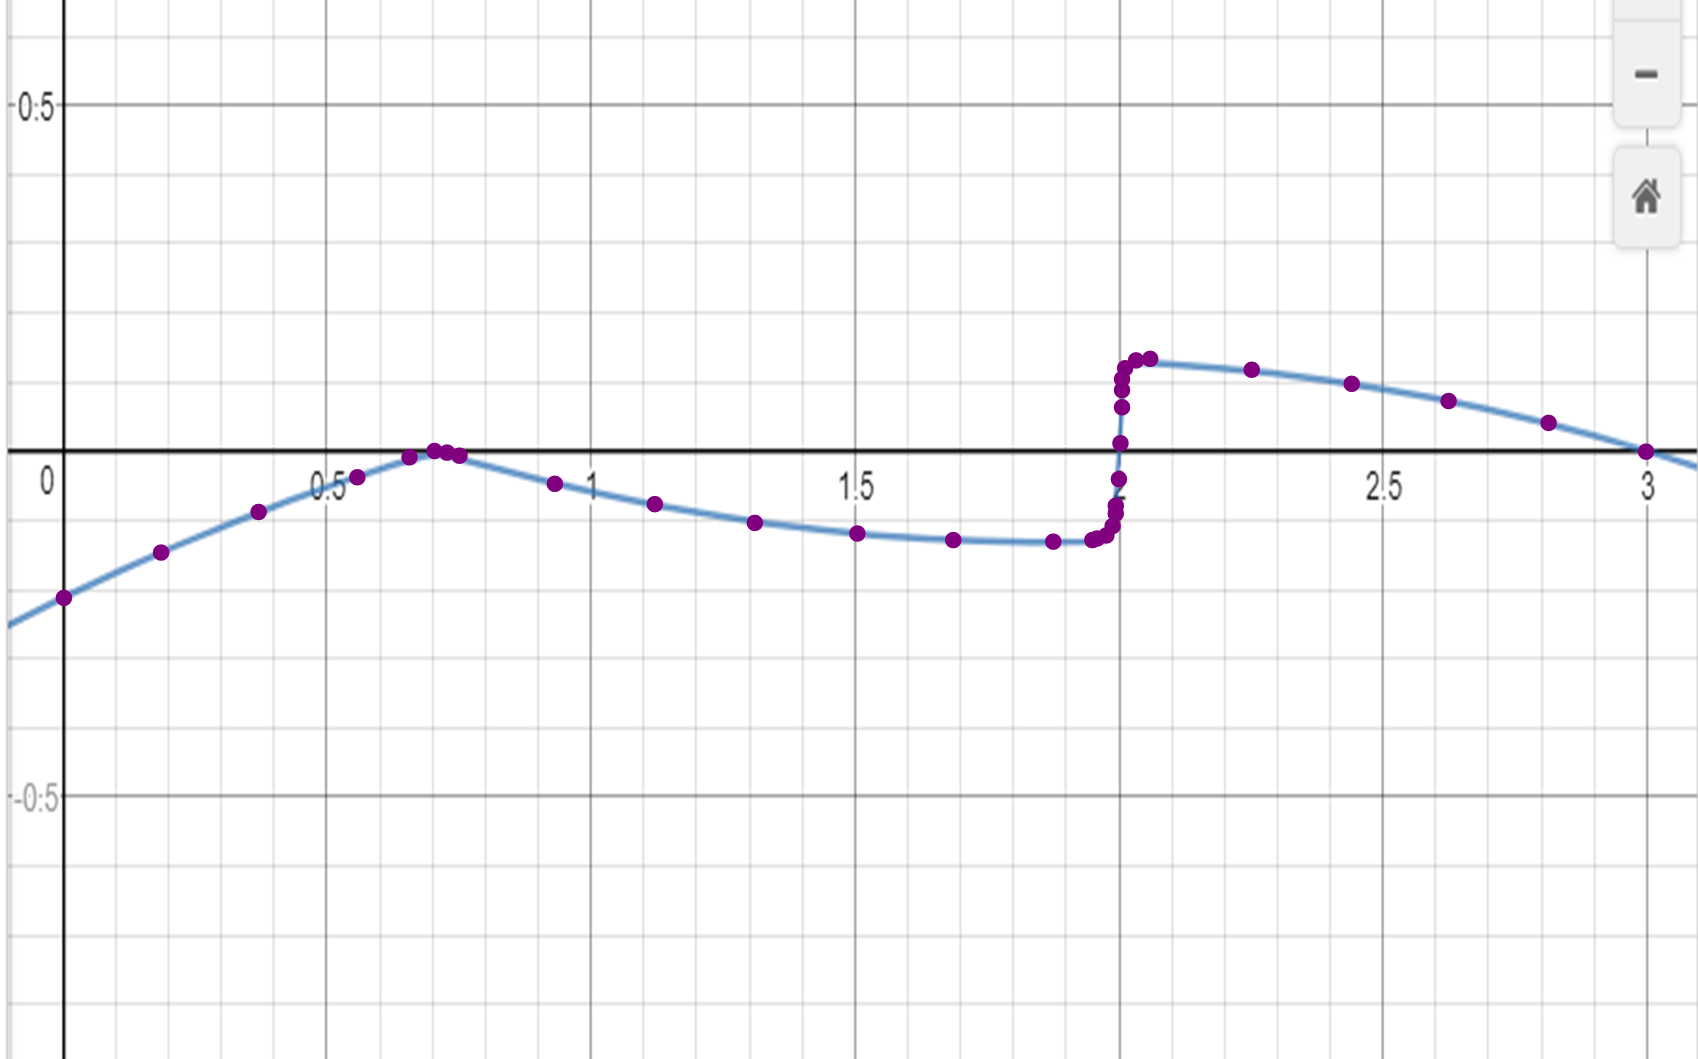
\includegraphics[scale=0.5]{OptimalMesh.png} 

\subsection*{Problem 2.d}

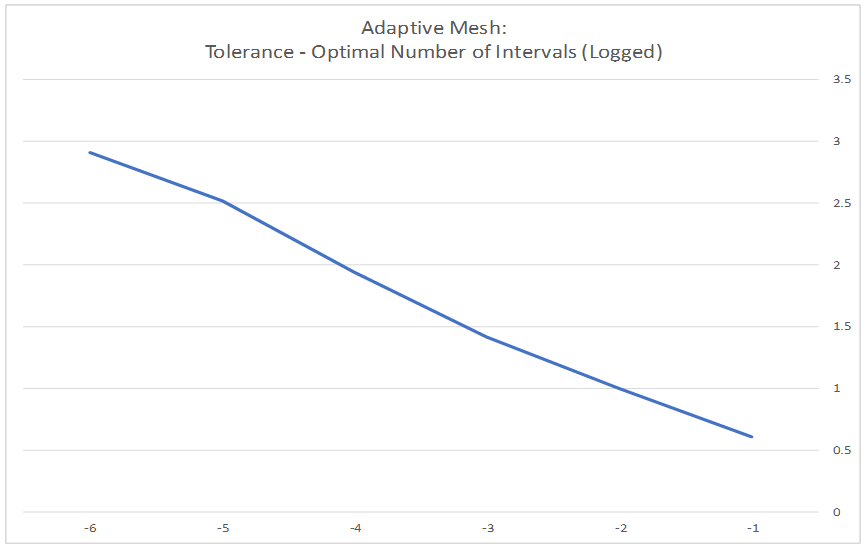
\includegraphics[scale=1]{Adaptive.png} 

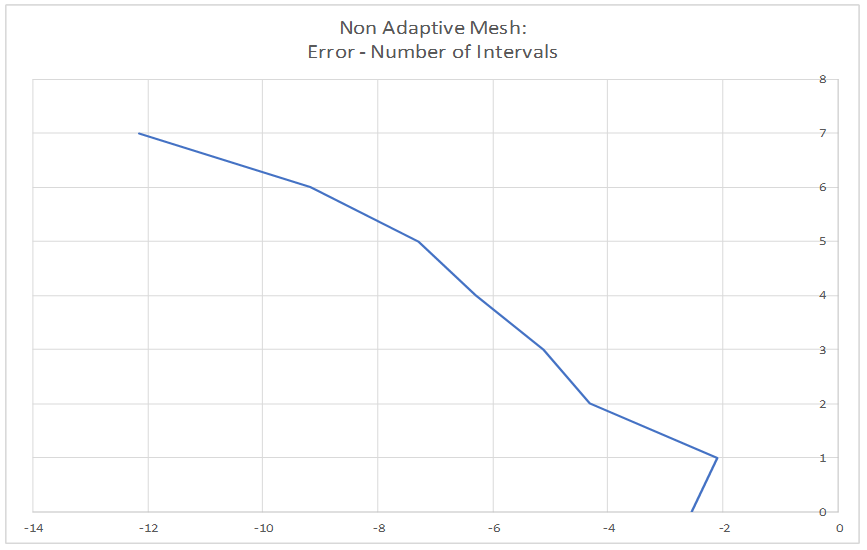
\includegraphics[scale=1]{NonAdaptive.png} 

\begin{verbatim}
Taking logs (base 10) of both the number of intervals and the tolerance of the 
adaptive mesh method I found that when I plotted the graph the gradient was around -2. 
When I took logs (base 2) of the number of intervals and the error with 
CGQ3 I found that the gradient was around -1/2

\end{verbatim}



%-----------------------------------------------------------------------------%
\end{document}
%-----------------------------------------------------------------------------%
